\documentclass[a4paper, 12pt]{article}
\usepackage{amsmath}
\usepackage[utf8]{inputenc}
\usepackage{graphicx}
\usepackage[left=2cm, right=2cm, bottom=3cm, top=2cm]{geometry}
\usepackage{natbib}
\usepackage{microtype}
\usepackage{minted}

\newcommand{\given}{\,|\,}

\title{Question Set 3 --- Parameter Estimation\\Solutions}
\author{}
\date{}

\begin{document}
\maketitle

%\abstract{\noindent Abstract}

% Need this after the abstract
\setlength{\parindent}{0pt}
\setlength{\parskip}{8pt}

\section*{Question 1}

There are two ways to approach this. One is to consider the three
hypotheses, $\eta=0$, $\eta=1$, $\eta=2$ in turn, and to assign
likelihoods by direct reasoning, like in the first set of questions.
However, since this is in the parameter estimation section, I'll use
a more parameter-estimation-y style here.

First, the prior for $\eta$ is uniform over its parameter
space $\{0,1,2\}$. To be lazy, we can just write
this as
\begin{align}
p(\eta) &\propto 1.
\end{align}

We can think of the data as being the number of `successes'
out of just one `trial' of an experiment where a toy is chosen
and tested for drugs. If success means drugs were found,
and failure means drugs were not found, then the
sampling distribution for the number of successes out of the
single trial is
\begin{align}
x | \eta \sim \textnormal{Binomial}\left(1, \frac{\eta}{2}\right).
\end{align}
The binomial distribution in this case reduces to
\begin{align}
p(x | \eta) &= (\eta/2)^x(1 - \eta/2)^{1-x}.
\end{align}
The observed value of $x$ was zero --- the result of the experiment
was zero successes out of one trial. Therefore the posterior is
\begin{align}
p(\eta | x) &\propto p(\eta)p(x|\eta)\\
            &= 1 \times (\eta/2)^0(1 - \eta/2)^{1} \\
            &\propto (1 - \eta/2).
\end{align}
This holds over the discrete parameter space $\{0,1,2\}$. Normalising
the posterior gives probabilities $\left\{\frac{2}{3}, \frac{1}{3} ,0\right\}$.

\section*{Question 2}
I'll do things analytically, except for the plot. The likelihood
is given in the question and the prior is an improper log-uniform
distribution:
\begin{align}
p(\lambda) &\propto \lambda^{-1}.
\end{align}
By Bayes' rule, the posterior is proportional to the prior times
the likelihood, i.e.,
\begin{align}
p(\lambda) &\propto \lambda^{-1} \times \lambda^5 e^{-\lambda} \\
           &\propto \lambda^4 e^{-\lambda}
\end{align}
where I have dropped the denominator from the likelihood because it
is a factor that does not depend on $\lambda$.
It's really easy to plot the un-normalised posterior in
Python. You can also normalise it numerically if you like.

\begin{minted}{python}
import numpy as np
import matplotlib.pyplot as plt

# Lambda grid
lamb = np.linspace(0.0, 20.0, 10001)

# Un-normalised posterior
post = lamb**4 * np.exp(-lamb)

# Plot
plt.plot(lamb, post)
plt.xlabel("$\\lambda$")
plt.show()
\end{minted}

Here is my plot of the un-normalised posterior.
By the way, it's a gamma distribution!:

\begin{figure}[!ht]
\centering
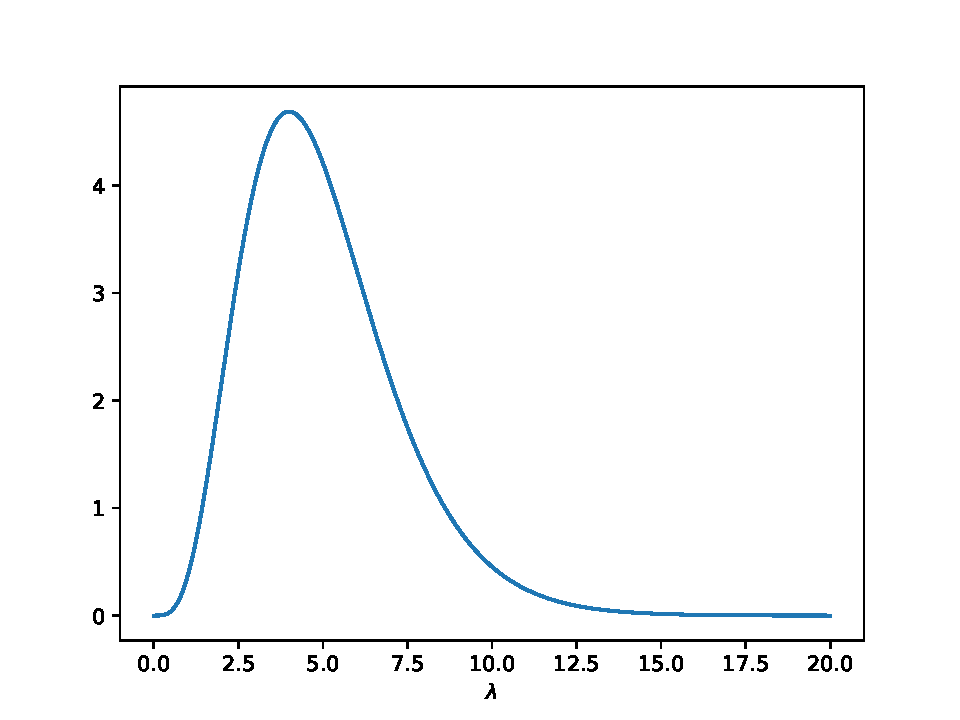
\includegraphics[width=0.7\textwidth]{gamma.pdf}
\end{figure}

\section*{Question 3}
Since I didn't teach prediction, I don't expect this to be obvious. You
might recognise some of the steps from Coryn's lectures, though.

Let $x'$ be the `next' data point. We want to know $x'$, and we do know
$x$. Therefore, it would be good to get the distribution
\begin{align}
p(x' | x)
\end{align}
and that is what we will get --- it's called a `posterior predictive
distribution'. We can get it by introducing $\lambda$, and
then marginalising it out again, i.e., by writing $p(x'|x)$ as
the marginal distribution of $x'$ that you would obtain from
the joint distribution of $x'$ and $\lambda$:
\begin{align}
p(x' | x) &= \int p(x', \lambda \,|\, x) \, d\lambda.
\end{align}
The next step is to use the product rule to decompose the joint
distribution inside the integral. It becomes a product of two terms,
one of which is the posterior which we already have, and the other
is the distribution we {\em would} use to predict $x'$ {\em if we
in fact knew $\lambda$} --- ultimately, a Poisson distribution
(this also assumes conditional independence).
\begin{align}
p(x' | x) &= \int p(\lambda | x)p(x' | \lambda, x) \, d\lambda \\
          &= \int p(\lambda | x)p(x' | \lambda) \, d\lambda \\
          &= \int p(\lambda | x) \frac{\lambda^{x!}e^{-\lambda}}{x'!} \, d\lambda.
\end{align}

I'll now compute this numerically:

\begin{minted}{python}
# Normalise the posterior
post = post / np.trapz(post, x=lamb)

# Lambda spacing for integration purposes
dl = lamb[1] - lamb[0]

# Set of possibilities for new data
x_prime = np.arange(0, 20)
predictive = np.zeros(len(x_prime))

# Needed for factorial
import scipy
import scipy.misc

# Loop over lambda values, accumulating the integral
for i in range(len(lamb)):
    predictive += dl*post[i]*lamb[i]**x_prime*np.exp(-lamb[i])\
                    /scipy.misc.factorial(x_prime)

# Plot the posterior predictive distribution
plt.bar(x_prime, predictive, alpha=0.2,
        label="Posterior predictive")

# Plot what it would be if we assumed the maximum likelihood
# estimate of lambda (5) was true
plt.bar(x_prime,
        5.0**x_prime*np.exp(-5.0)/scipy.misc.factorial(x_prime),
        alpha=0.1, label="Based on $\\hat{\\lambda}=5$")
plt.xlabel("$x'$")
plt.ylabel("Probability")
plt.legend()
plt.show()
\end{minted}

Here is the plot:

\begin{figure}[!ht]
\centering
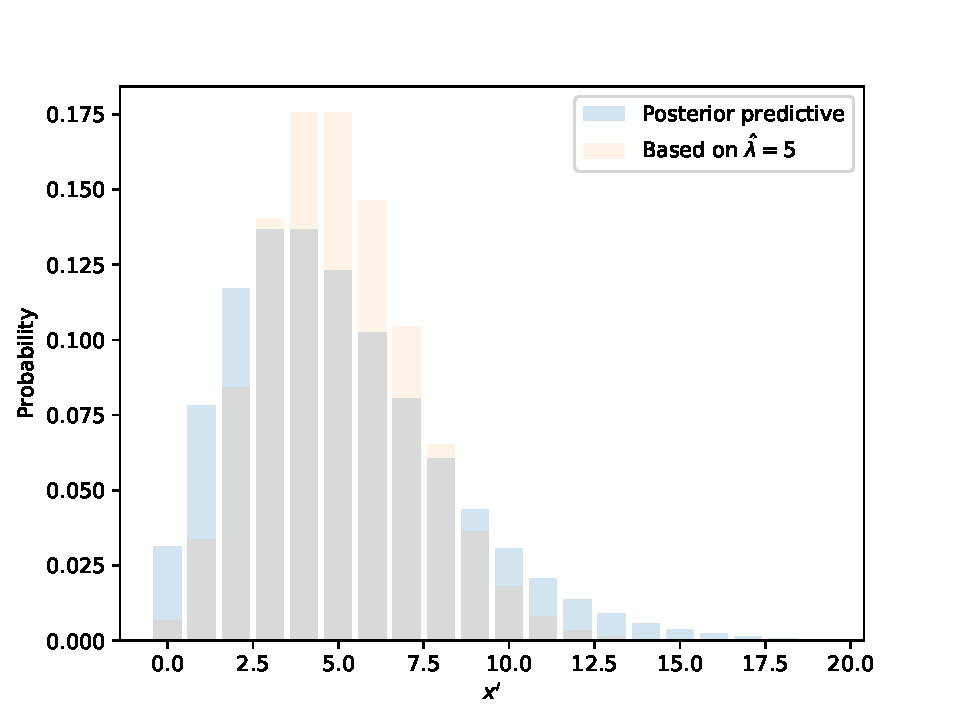
\includegraphics[width=0.7\textwidth]{predictive.pdf}
\end{figure}

The Bayesian predictive distribution has heavier tails because
it incorporates the reality that $\lambda$ is not known
precisely.

\end{document}

